\documentclass{standalone}
\usepackage{tikz}
\usepackage{tkz-graph}
\usepackage{tkz-berge}

\begin{document}

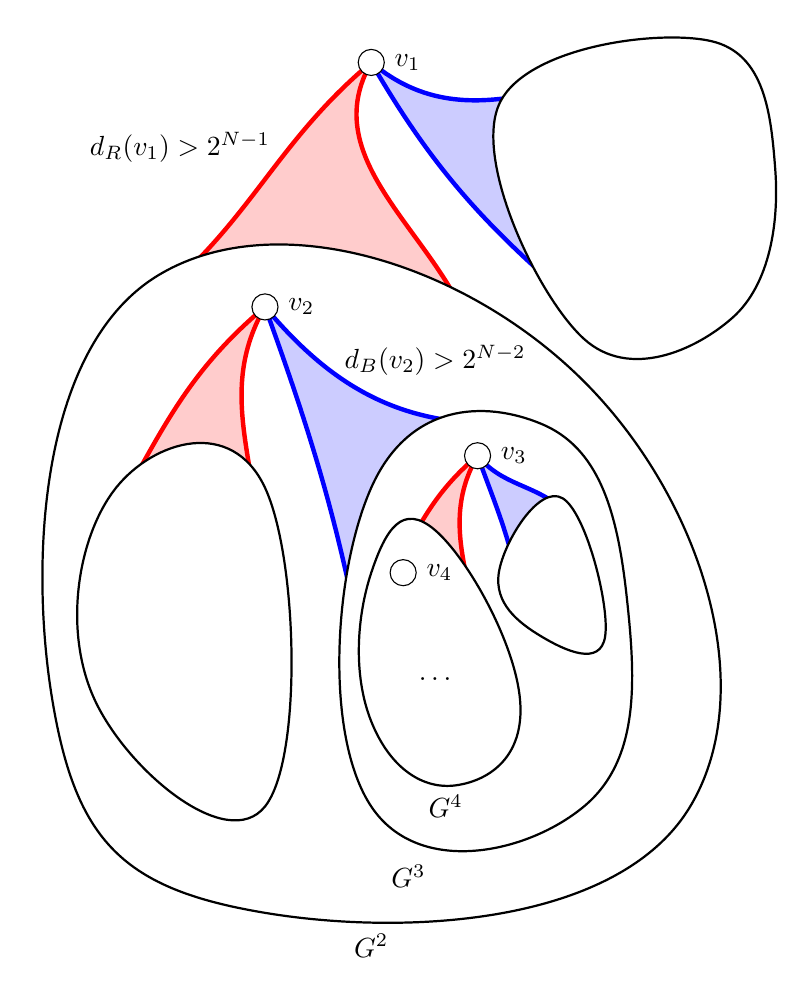
\begin{tikzpicture}[scale=2.7]
  \tikzstyle{vertex}=[circle,draw=black,fill=white,minimum size=8pt];
  \tikzstyle{region}=[fill=white,thick]

  \draw [red, ultra thick, fill=red!20] (-2.0,0.5) to [out=220, in=40] (-3.0,-0.6) -- (-1.5,-1.1) to [out=80,in=240] (-2.0,0.5);
  \draw [blue, ultra thick, fill=blue!20] (-2.0,0.5) to [out=-40, in=180] (-0.4,0.5) -- (-0.9,-0.75) to [out=140,in=-60] (-2.0,0.5);

  \node[vertex] (v1) at (-2.0,0.5) [label=right:$v_1$] {};

  \draw[region] plot [smooth cycle, tension=0.8] coordinates {(-1,-1) (-3,-0.5) (-3.5,-2.5) (-2.5,-3.5) (-0.5,-3)};
  \draw[region] plot [smooth cycle, tension=0.7] coordinates {(-1.4,0.3) (-0.4,0.6) (-0.1,0) (-0.3,-0.7) (-1.0,-0.8)};

  \node (d1) at (-2.9,0.1) {$d_R(v_1) > 2^{N-1}$};
  \node (nr1) at (-2.0,-3.655) {$G^2$};
  %\node (nr1) at (-2.0,-3.655) {$N_R(v_1)$};
  %\node (nb1) at (-0.5,-1.05) {$N_B(v_1)$};

  \draw [red, ultra thick, fill=red!20] (-2.5,-0.65) to [out=220, in=60] (-3.25,-1.7) -- (-2.55,-2) to [out=80,in=240] (-2.5,-0.65);
  \draw [blue, ultra thick, fill=blue!20] (-2.5,-0.65) to [out=-50, in=180] (-1.4,-1.2) -- (-2.0,-2.5) to [out=100,in=-70] (-2.5,-0.65);

  \node[vertex] (v2) at (-2.5,-0.65) [label=right:$v_2$] {};

  \draw[region] plot [smooth cycle, tension=0.8] coordinates {(-3.2,-1.5) (-3.3,-2.5) (-2.5,-3.0) (-2.5,-1.5)};
  \draw[region] plot [smooth cycle, tension=0.8] coordinates {(-1.2,-1.2) (-0.8,-2.0) (-1.0, -3.0) (-2.0,-3.0) (-2.0,-1.5)};

  \node (d1) at (-1.7,-0.9) {$d_B(v_2) > 2^{N-2}$};
  %\node (nr2) at (-2.7,-3.2) {$N_R(v_2)$};
  %\node (nb2) at (-1.3,-3.3) {$N_B(v_2)$};
  \node (nb2) at (-1.825,-3.3275) {$G^3$};



  \draw [red, ultra thick, fill=red!20] (-1.5,-1.35) to [out=220, in=60] (-1.95,-2.0) -- (-1.5,-2.5) to [out=80,in=240] (-1.5,-1.35);
  \draw [blue, ultra thick, fill=blue!20] (-1.5,-1.35) to [out=-50, in=140] (-1.1,-1.6) -- (-1.3,-2) to [out=100,in=-70] (-1.5,-1.35);

  \node[vertex] (v3) at (-1.5,-1.35) [label=right:$v_3$] {};

  \draw[region] plot [smooth cycle, tension=0.8] coordinates {(-1.7,-1.7) (-1.3,-2.5) (-1.6, -2.9) (-2.0,-2.6) (-2.0,-1.9)};
  \draw[region] plot [smooth cycle, tension=0.8] coordinates {(-1.1,-1.55) (-0.9,-2.2) (-1.2, -2.2) (-1.4,-1.9)};

  %\node (nr3) at (-1.65,-3.0) {$N_R(v_3)$};
  %\node (nb3) at (-1.05,-2.4) {$N_B(v_3)$};
  \node (nr3) at (-1.65,-3.0) {$G^4$};

  \node[vertex] (v4) at (-1.85,-1.9) [label=right:$v_4$] {};
  \node(ret2) at (-1.7,-2.4) {$\dots$};

\end{tikzpicture}

\end{document}
